\FloatBarrier
\subsection{Loss Cone}\label{sec:losscone}

Assuming a dipolar geomagnetic field, reasonable for altitudes $h < 3 R_E$, the McIlwain L-shell
\begin{equation}\label{eq:Lshell}
L = \frac{r_e}{R_E}
%\marginnote{L-shell number}
\end{equation}
where $r_e$ is the geocentric distance to the point where the $B$ field line crosses the magnetic equator is a convenient parameter for describing near-Earth magnetospheric phenomena.
As L increases, eventually the magnetopause and open field lines are reached leading into the solar wind.
As L decreases, the collisions increase such that the particle behavior becomes collision dominated for small L.
The geocentric distance to a mirroring particle is
\begin{equation}
r=L \cos^2 \lambda
\end{equation}
where $\lambda$ is the magnetic latitude of the field line.
To obtain invariant latitude, that is the magnetic latitude where an L-shell intersects the Earth's surface, plug in $r=R_E, \lambda=\lambda_E, r_0=L R_E$ \citep{kivelson}
\begin{equation}
\Lambda = \cos^{-1} \sqrt{\frac{1}{L}}.
\end{equation}
The particle will be lost if 
\begin{equation}
\alpha_p \leq \sin^{-1}\left(4L^6 - 3 L^5\right)^{-1/4}
\end{equation}
as depicted in the blue area in Figure~\ref{fig:losscone}.
\begin{figure}\centering
	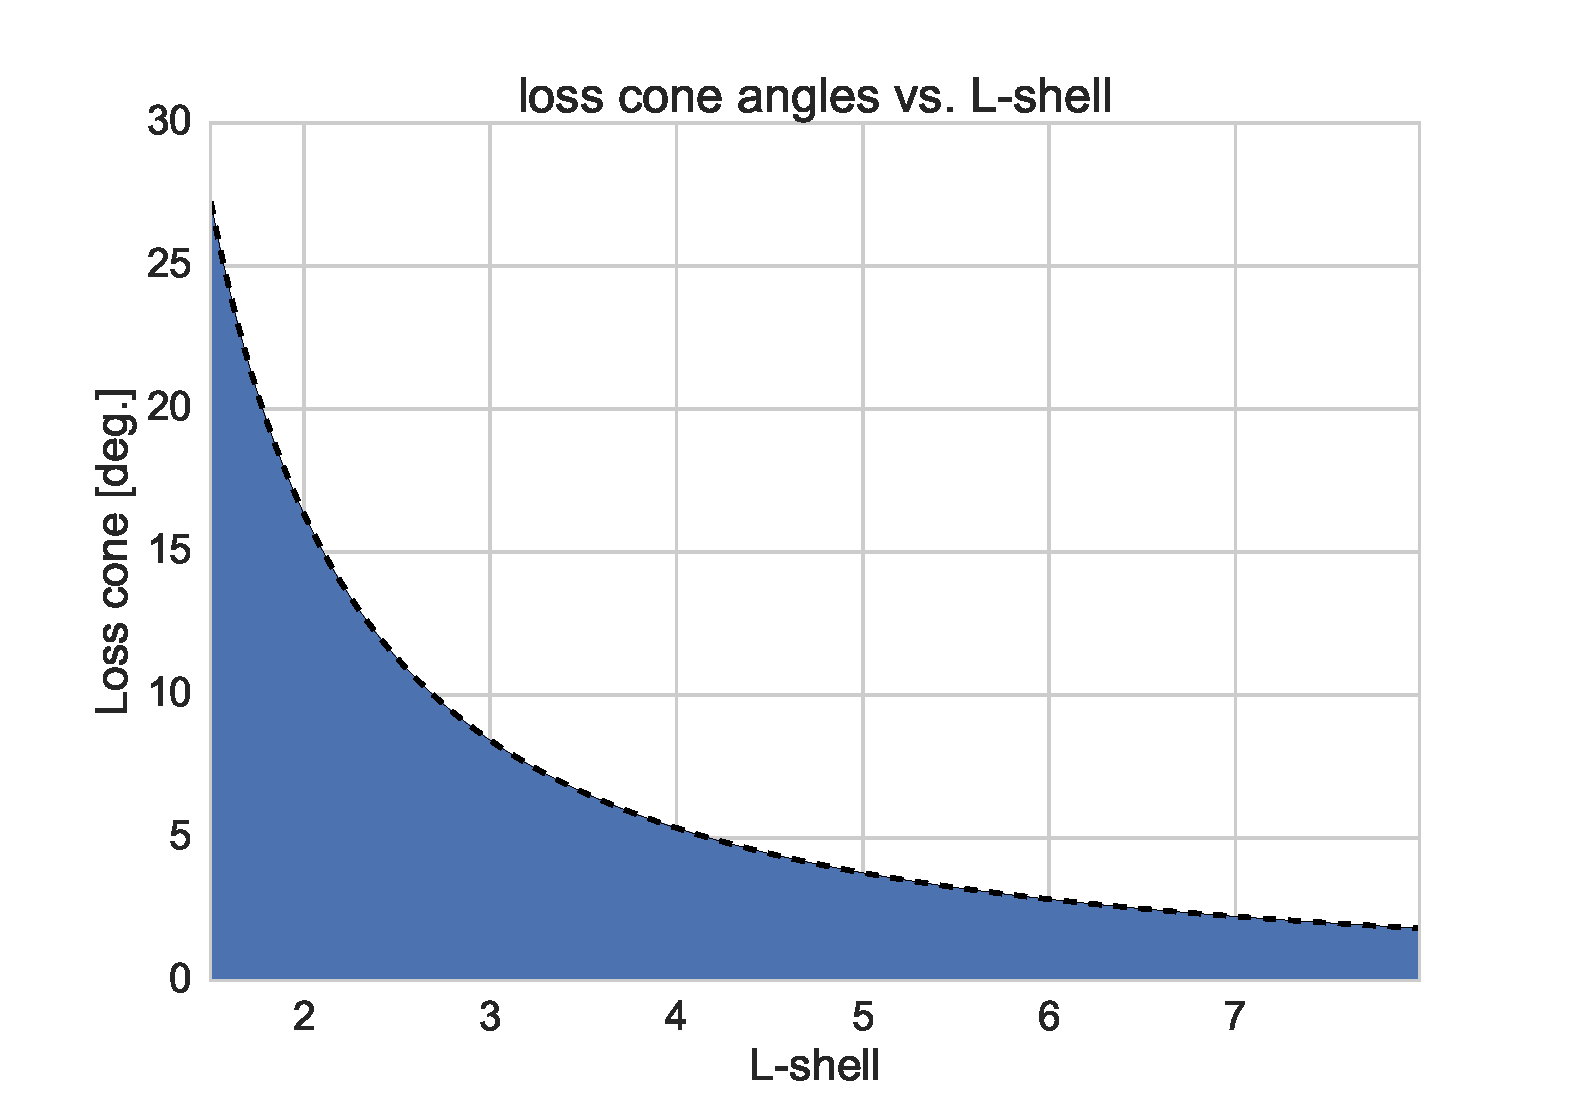
\includegraphics[width=0.8\linewidth]{gfx/lossconeangle}
	\caption{Shaded area indicates loss cone width vs. L-shell}\label{fig:losscone}
\end{figure}
Mirroring particles that are accelerated along $B$ experience an increase in $v_\parallel$ and a decrease in $\alpha_p$, increasing the likelihood the accelerated population will precipitate into the ionosphere and create aurora.
Some important L-shells for Earth are:
\begin{itemize}
	\item nightside plasmapause: 3.5 (active) to 5 (quiet)
	\item inner Van Allen Belt: 1.03 (SAA) to 3
	\item auroral oval: 4..6
\end{itemize}